\documentclass[11pt,a4paper]{report}
\usepackage[textwidth=37em,vmargin=30mm]{geometry}
\usepackage{calc,xunicode,amsmath,amssymb,paralist,enumitem,tabu,booktabs,datetime2,xeCJK,xeCJKfntef,listings}
\usepackage{tocloft,fancyhdr,tcolorbox,xcolor,graphicx,eso-pic,xltxtra,xelatexemoji}

\newcommand{\envyear}[0]{2024}
\newcommand{\envdatestr}[0]{2024-10-18}
\newcommand{\envfinaldir}[0]{webdb/2024/20241018/final}

\usepackage[hidelinks]{hyperref}
\hypersetup{
    colorlinks=false,
    pdfpagemode=FullScreen,
    pdftitle={Web Digest - \envdatestr}
}

\setlength{\cftbeforechapskip}{10pt}
\renewcommand{\cftchapfont}{\rmfamily\bfseries\large\raggedright}
\setlength{\cftbeforesecskip}{2pt}
\renewcommand{\cftsecfont}{\sffamily\small\raggedright}

\setdefaultleftmargin{2em}{2em}{1em}{1em}{1em}{1em}

\usepackage{xeCJK,xeCJKfntef}
\xeCJKsetup{PunctStyle=plain,RubberPunctSkip=false,CJKglue=\strut\hskip 0pt plus 0.1em minus 0.05em,CJKecglue=\strut\hskip 0.22em plus 0.2em}
\XeTeXlinebreaklocale "zh"
\XeTeXlinebreakskip = 0pt


\setmainfont{Brygada 1918}
\setromanfont{Brygada 1918}
\setsansfont{IBM Plex Sans}
\setmonofont{JetBrains Mono NL}
\setCJKmainfont{Noto Serif CJK SC}
\setCJKromanfont{Noto Serif CJK SC}
\setCJKsansfont{Noto Sans CJK SC}
\setCJKmonofont{Noto Sans CJK SC}

\setlength{\parindent}{0pt}
\setlength{\parskip}{8pt}
\linespread{1.15}

\lstset{
	basicstyle=\ttfamily\footnotesize,
	numbersep=5pt,
	backgroundcolor=\color{black!5},
	showspaces=false,
	showstringspaces=false,
	showtabs=false,
	tabsize=2,
	captionpos=b,
	breaklines=true,
	breakatwhitespace=true,
	breakautoindent=true,
	linewidth=\textwidth
}






\newcommand{\coverpic}[2]{
    % argv: itemurl, authorname
    Cover photo by #2~~(\href{#1}{#1})
}
\newcommand{\makeheader}[0]{
    \begin{titlepage}
        % \newgeometry{hmargin=15mm,tmargin=21mm,bmargin=12mm}
        \begin{center}
            
            \rmfamily\scshape
            \fontspec{BaskervilleF}
            \fontspec{Old Standard}
            \fontsize{59pt}{70pt}\selectfont
            WEB\hfill DIGEST
            
            \vfill
            % \vskip 30pt
            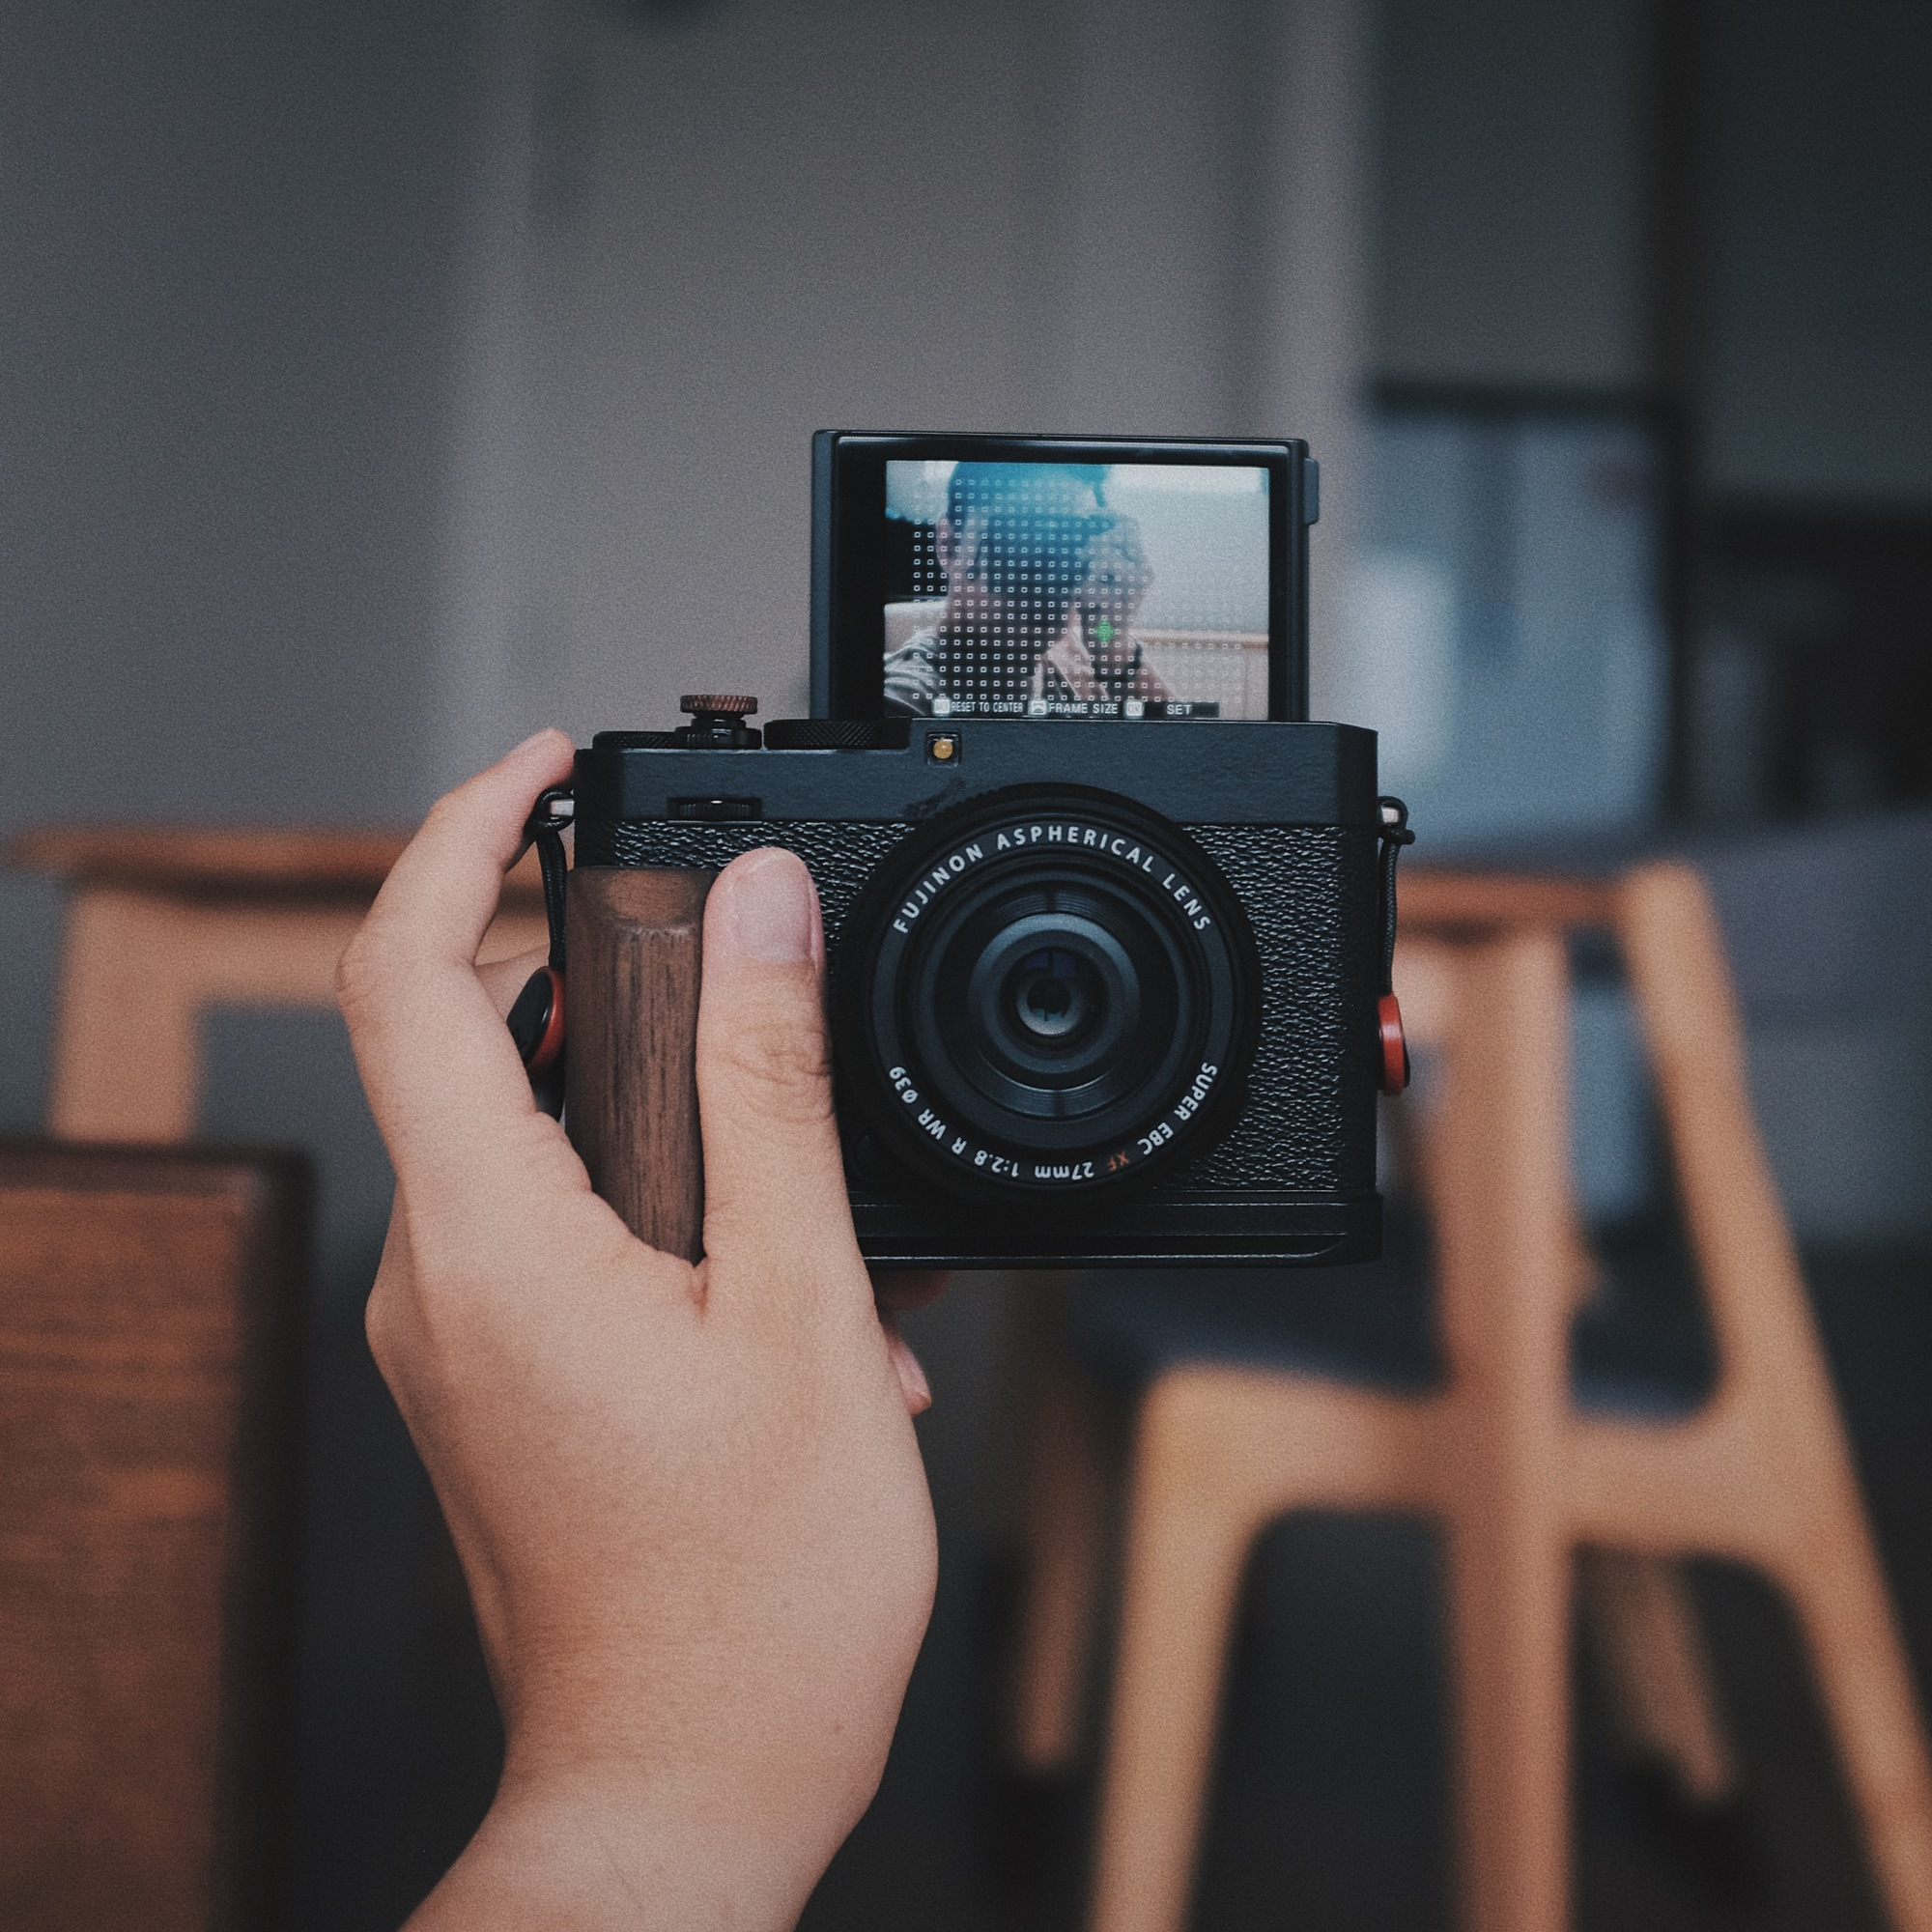
\includegraphics[width=\linewidth]{\envfinaldir/coverpic-prod.jpg}\par
            % \vskip 30pt
            \vfill

            \normalsize\rmfamily\scshape
            \copyright{} The Web Digest Project \hfill\large \envdatestr
        \end{center}
    \end{titlepage}
    % \restoregeometry
}
\newcommand{\simplehref}[1]{%
    \textcolor{blue!80!green}{\href{#1}{#1}}%
}
\renewcommand{\contentsname}{\center\Huge\sffamily\bfseries Contents\par\vskip 20pt}
\newcounter{ipartcounter}
\setcounter{ipartcounter}{0}
\newcommand{\ipart}[1]{
    % \vskip 20pt
    \clearpage
    \stepcounter{ipartcounter}
    \phantomsection
    \addcontentsline{toc}{chapter}{#1}
    % \begin{center}
    %     \Huge
    %     \sffamily\bfseries
    %     #1
    % \end{center}
    % \vskip 20pt plus 7pt
}
\newcounter{ichaptercounter}
\setcounter{ichaptercounter}{0}
\newcommand{\ichapter}[1]{
    % \vskip 20pt
    \clearpage
    \stepcounter{ichaptercounter}
    \phantomsection
    \addcontentsline{toc}{section}{\numberline{\arabic{ichaptercounter}}#1}
    \begin{center}
        \Huge
        \sffamily\bfseries
        #1
    \end{center}
    \vskip 20pt plus 7pt
}
\newcommand{\entrytitlefont}[1]{\subsection*{\raggedright\Large\sffamily\bfseries#1}}
\newcommand{\entryitemGeneric}[2]{
    % argv: title, url
    \parbox{\linewidth}{
        \entrytitlefont{#1}\par\vskip 5pt
        \footnotesize\ttfamily\mdseries
        \simplehref{#2}
    }\vskip 11pt plus 11pt minus 1pt
}
\newcommand{\entryitemGithub}[3]{
    % argv: title, url, desc
    \parbox{\linewidth}{
        \entrytitlefont{#1}\par\vskip 5pt
        \footnotesize\ttfamily\mdseries
        \simplehref{#2}\par\vskip 5pt
        \small\rmfamily\mdseries#3
    }\vskip 11pt plus 11pt minus 1pt
}
\newcommand{\entryitemAp}[3]{
    % argv: title, url, desc
    \parbox{\linewidth}{
        \entrytitlefont{#1}\par\vskip 5pt
        \footnotesize\ttfamily\mdseries
        \simplehref{#2}\par\vskip 5pt
        \small\rmfamily\mdseries#3
    }\vskip 11pt plus 11pt minus 1pt
}
\newcommand{\entryitemHackernews}[3]{
    % argv: title, hnurl, rawurl
    % \parbox{\linewidth}{
    %     \entrytitlefont{#1}\par\vskip 5pt
    %     \footnotesize\ttfamily\mdseries
    %     \simplehref{#3}\par
    %     \textcolor{black!50}{\href{#2}{#2}}
    % }\vskip 11pt plus 11pt minus 1pt
    \begin{minipage}{\linewidth}
            \entrytitlefont{#1}\par\vskip 5pt
            \footnotesize\ttfamily\mdseries
            \simplehref{#3}\par
            \textcolor{black!50}{\href{#2}{#2}}
    \end{minipage}\par\vskip 11pt plus 11pt minus 1pt
}







\begin{document}

\makeheader

\tableofcontents\clearpage




\ipart{Developers}
\ichapter{Hacker News}
\entryitemTwoLinks{Kagi Update: AI Image Filter for Search Results}{https://news.ycombinator.com/item?id=41873204}{https://help.kagi.com/kagi/features/exclude-ai-images.html}

\entryitemTwoLinks{Is Matt Mullenweg defending WordPress or sabotaging it?}{https://news.ycombinator.com/item?id=41872628}{https://torment-nexus.mathewingram.com/is-matt-mullenweg-defending-wordpress-or-sabotaging-it/}

\entryitemTwoLinks{Employees Describe an Environment of Paranoia and Fear Inside Automattic}{https://news.ycombinator.com/item?id=41872046}{https://www.404media.co/automattic-buyout-offer-wordpress-matt-mullenweg/}

\entryitemTwoLinks{Qualcomm cancels Snapdragon Dev Kit, refunds all orders}{https://news.ycombinator.com/item?id=41871899}{https://www.jeffgeerling.com/blog/2024/qualcomm-cancels-snapdragon-dev-kit-refunds-all-orders}

\entryitemTwoLinks{Crokinole}{https://news.ycombinator.com/item?id=41871375}{https://pudding.cool/2024/10/crokinole/}

\entryitemTwoLinks{NotebookLM launches feature to customize and guide audio overviews}{https://news.ycombinator.com/item?id=41871262}{https://blog.google/technology/ai/notebooklm-update-october-2024/}

\entryitemTwoLinks{I'm Peter Roberts, immigration attorney who does work for YC and startups. AMA}{https://news.ycombinator.com/item?id=41870887}{https://news.ycombinator.com/item?id=41870887}

\entryitemTwoLinks{Adobe's new image rotation tool is one of the most impressive AI tools seen}{https://news.ycombinator.com/item?id=41870040}{https://www.creativebloq.com/design/adobes-new-image-rotation-tool-is-one-of-the-most-impressive-ai-concepts-weve-seen}

\entryitemTwoLinks{Gamedev in Lisp. Part 2: Dungeons and Interfaces}{https://news.ycombinator.com/item?id=41869460}{https://gitlab.com/lockie/cl-fast-ecs/-/wikis/tutorial-2}

\entryitemTwoLinks{Cats are (almost) liquid}{https://news.ycombinator.com/item?id=41868683}{https://www.cell.com/iscience/fulltext/S2589-0042(24)02024-8}

\entryitemTwoLinks{Escaping the Chrome Sandbox Through DevTools}{https://news.ycombinator.com/item?id=41866802}{https://ading.dev/blog/posts/chrome\_sandbox\_escape.html}

\entryitemTwoLinks{OpenVMM – A New VMM for Windows and Linux, Written in Rust}{https://news.ycombinator.com/item?id=41866742}{https://github.com/microsoft/openvmm}

\entryitemTwoLinks{WordPress retaliation impacts community}{https://news.ycombinator.com/item?id=41866328}{https://lwn.net/SubscriberLink/993895/c0438e0ee9382c5f/}

\entryitemTwoLinks{Using Cloudflare on your website could be blocking RSS users}{https://news.ycombinator.com/item?id=41864632}{https://openrss.org/blog/using-cloudflare-on-your-website-could-be-blocking-rss-users}

\entryitemTwoLinks{Show HN: Automated smooth Nth order derivatives of noisy data}{https://news.ycombinator.com/item?id=41863398}{https://github.com/hugohadfield/kalmangrad}

\entryitemTwoLinks{Should We Chat, Too? Security Analysis of WeChat's Mmtls Encryption Protocol}{https://news.ycombinator.com/item?id=41863278}{https://citizenlab.ca/2024/10/should-we-chat-too-security-analysis-of-wechats-mmtls-encryption-protocol/}

\entryitemTwoLinks{AI PCs Aren't Good at AI: The CPU Beats the NPU}{https://news.ycombinator.com/item?id=41863061}{https://github.com/usefulsensors/qc\_npu\_benchmark}

\entryitemTwoLinks{We outsmarted CSGO cheaters with IdentityLogger}{https://news.ycombinator.com/item?id=41862028}{https://mobeigi.com/blog/gaming/how-we-outsmarted-csgo-cheaters-with-identitylogger/}

\entryitemTwoLinks{Ireland's big school secret: how a year off-curriculum changes teenage lives}{https://news.ycombinator.com/item?id=41861628}{https://www.theguardian.com/lifeandstyle/2024/oct/16/ireland-school-secret-transition-year-off-curriculum}

\entryitemTwoLinks{Optimizing the Ion compiler back end}{https://news.ycombinator.com/item?id=41861442}{https://spidermonkey.dev/blog/2024/10/16/75x-faster-optimizing-the-ion-compiler-backend.html}\ichapter{Phoronix}
\entryitemGeneric{\hskip 0pt{}Intel NPU Driver Being Updated To Handle Larger AI Workloads}{https://www.phoronix.com/news/Intel-NPU-Bigger-Workloads}

\entryitemGeneric{\hskip 0pt{}Exploring The Zen 5 SMT Performance With The AMD EPYC 9755 "Turin" CPU}{https://www.phoronix.com/review/amd-epyc-9755-smt}

\entryitemGeneric{\hskip 0pt{}PyTorch 2.5 Released With Improved Intel GPU Support}{https://www.phoronix.com/news/PyTorch-2.5-Released}

\entryitemGeneric{\hskip 0pt{}Red Hat Engineer Nikita Popov Now The Lead Maintainer For LLVM}{https://www.phoronix.com/news/LLVM-Lead-Maintainer-Popov}

\entryitemGeneric{\hskip 0pt{}Linux 6.13 To Introduce Intel 5th Gen NPU Support For Panther Lake}{https://www.phoronix.com/news/Intel-PantherLake-NPU-Linux-613}

\entryitemGeneric{\hskip 0pt{}The Maturing State Of Rusticl For Rust-Based OpenCL Within Mesa}{https://www.phoronix.com/news/Rusticl-2024-Status-Update}

\entryitemGeneric{\hskip 0pt{}AMD Working On GPU Compute Virtualization Support With ROCm/HIP For VMs}{https://www.phoronix.com/news/AMD-ROCm-HIP-For-VMs-Coming}

\entryitemGeneric{\hskip 0pt{}OGRE-Next 3.0 Released For This Open-Source 3D Engine}{https://www.phoronix.com/news/OGRE-Next-3.0}

\entryitemGeneric{\hskip 0pt{}AMD Releases AOMP 20.0-0 For Radeon/Instinct Compiler Offloading}{https://www.phoronix.com/news/AMD-AOMP-20.0-0-Compiler}


\ipart{Developers~~~~(zh-Hans)}
\ichapter{Solidot}
\entryitemGeneric{\hskip 0pt{}Matt Mullenweg 的报复行动冲击 WordPress 社区}{https://www.solidot.org/story?sid=79520}

\entryitemGeneric{\hskip 0pt{}哈勃发现木星大红斑大小会变化}{https://www.solidot.org/story?sid=79519}

\entryitemGeneric{\hskip 0pt{}官方机构指责英特尔产品存在网络安全问题}{https://www.solidot.org/story?sid=79518}

\entryitemGeneric{\hskip 0pt{}Twitter/X 将使用用户帖子训练 AI,这一次用户无法退出}{https://www.solidot.org/story?sid=79517}

\entryitemGeneric{\hskip 0pt{}腾讯微信使用的 MMTLS 加密协议存在安全弱点}{https://www.solidot.org/story?sid=79516}

\entryitemGeneric{\hskip 0pt{}高收入的低稳定性}{https://www.solidot.org/story?sid=79515}

\entryitemGeneric{\hskip 0pt{}Winamp 移除源码库}{https://www.solidot.org/story?sid=79514}

\entryitemGeneric{\hskip 0pt{}亚马逊宣布了彩屏 Kindle}{https://www.solidot.org/story?sid=79513}

\entryitemGeneric{\hskip 0pt{}FTC 宣布了简化取消订阅的规定}{https://www.solidot.org/story?sid=79512}

\entryitemGeneric{\hskip 0pt{}Google 计划在更多服务中使用 Rust 语言}{https://www.solidot.org/story?sid=79511}

\entryitemGeneric{\hskip 0pt{}用手游骗了数亿美元的男子面临 8.9 万年监禁}{https://www.solidot.org/story?sid=79510}

\entryitemGeneric{\hskip 0pt{}突触变化将多次获胜的小鼠变成恶霸}{https://www.solidot.org/story?sid=79509}

\entryitemGeneric{\hskip 0pt{}三季度智能手机出货量增长 4\%}{https://www.solidot.org/story?sid=79508}

\entryitemGeneric{\hskip 0pt{}青少年社媒使用与焦虑和抑郁强相关}{https://www.solidot.org/story?sid=79507}

\entryitemGeneric{\hskip 0pt{}日本继续工作的 65 岁以上老年人数量超 900 万}{https://www.solidot.org/story?sid=79506}

\entryitemGeneric{\hskip 0pt{}日本高滨核电站 1 号机组获准运行超过 50 年}{https://www.solidot.org/story?sid=79505}

\entryitemGeneric{\hskip 0pt{}太阳活动进入极大期}{https://www.solidot.org/story?sid=79504}

\entryitemGeneric{\hskip 0pt{}Google Chrome 开始自动禁用 uBlock Origin}{https://www.solidot.org/story?sid=79503}

\entryitemGeneric{\hskip 0pt{}诺贝尔经济学奖授予了证明制度对国家繁荣重要性的三位经济学家}{https://www.solidot.org/story?sid=79502}

\entryitemGeneric{\hskip 0pt{}AMD 和英特尔宣布在 x86 架构实现上展开合作}{https://www.solidot.org/story?sid=79501}\ichapter{V2EX}
\entryitemGeneric{\hskip 0pt{}[程序员] 求助: 前端开发能让用户自助添加/拖动/缩放小组件的仪表面板}{https://www.v2ex.com/t/1081353}

\entryitemGeneric{\hskip 0pt{}[分享发现] 💥iOS 应用 World Clock Master 永久内购首免啦!}{https://www.v2ex.com/t/1081351}

\entryitemGeneric{\hskip 0pt{}[Android] 港版三星使用国内 APP 如何保障 APP 的权限是符合标准的}{https://www.v2ex.com/t/1081350}

\entryitemGeneric{\hskip 0pt{}[程序员] Git for windows 2.47.0 克隆卡死}{https://www.v2ex.com/t/1081349}

\entryitemGeneric{\hskip 0pt{}[推广] 新西兰 Skinny Sim 卡 [已激活] 现货包邮 99 一张 [盖楼送卡]}{https://www.v2ex.com/t/1081348}

\entryitemGeneric{\hskip 0pt{}[程序员] 想利用闲暇时间,开发一个博客平台,有兴趣的童鞋请关注,欢迎贡献代码。}{https://www.v2ex.com/t/1081347}

\entryitemGeneric{\hskip 0pt{}[问与答] iPhone 手机浏览器上不了 v2ex.com}{https://www.v2ex.com/t/1081346}

\entryitemGeneric{\hskip 0pt{}[Apple] 求一款支持``Transcript''这个功能的视频播放器 app (Mac/ iPad )}{https://www.v2ex.com/t/1081345}

\entryitemGeneric{\hskip 0pt{}[程序员] 当面试官问为什么选择 Kafka/RabbitMQ/RocketMQ 时,他到底想问什么?}{https://www.v2ex.com/t/1081344}

\entryitemGeneric{\hskip 0pt{}[问与答] 推频繁永久封禁我的账号,这是被盯上了吗}{https://www.v2ex.com/t/1081342}

\entryitemGeneric{\hskip 0pt{}[程序员] 半夜了,诉苦一下吧,希望大家见谅}{https://www.v2ex.com/t/1081341}

\entryitemGeneric{\hskip 0pt{}[Apple] 2024 年 10 月蜂窝版 iPad mini 的选择, 6 还是 7?}{https://www.v2ex.com/t/1081338}

\entryitemGeneric{\hskip 0pt{}[问与答] 为什么同样的一段正则表达式, JS 和 Java 的匹配结果不一样呢?}{https://www.v2ex.com/t/1081336}

\entryitemGeneric{\hskip 0pt{}[分享创造] Canvas 编写的扫雷小游戏(点开即玩)}{https://www.v2ex.com/t/1081335}

\entryitemGeneric{\hskip 0pt{}[问与答] 程序员使用 wsl 2 有啥最佳实践么?}{https://www.v2ex.com/t/1081334}

\entryitemGeneric{\hskip 0pt{}[问与答] 小企业自建电商商城有哪些选项?}{https://www.v2ex.com/t/1081333}

\entryitemGeneric{\hskip 0pt{}[分享创造] 开源项目:当有人给你的 GitHub 项目 Star 时,自动发送通知到 Telegram。}{https://www.v2ex.com/t/1081332}

\entryitemGeneric{\hskip 0pt{}[问与答] 哪家代理支持 43 端口,且国外链接比较好?}{https://www.v2ex.com/t/1081331}

\entryitemGeneric{\hskip 0pt{}[科技] 微软将终止中国个人 Azure OpenAI 服务,仅企业客户可用}{https://www.v2ex.com/t/1081330}

\entryitemGeneric{\hskip 0pt{}[酷工作] Android 和 PC 渲染工程 地点:南京,薪资 20-45k}{https://www.v2ex.com/t/1081327}

\entryitemGeneric{\hskip 0pt{}[酷工作] [兼职] Kepler.gl 插件开发}{https://www.v2ex.com/t/1081326}

\entryitemGeneric{\hskip 0pt{}[求职] 招聘 Java 及安卓工程师,要求懂智能柜}{https://www.v2ex.com/t/1081325}

\entryitemGeneric{\hskip 0pt{}[问与答] Rust 移动有带来什么好处吗?}{https://www.v2ex.com/t/1081324}

\entryitemGeneric{\hskip 0pt{}[程序员] mod\_security 中的 SecUnicodeMapFile unicode.mapping}{https://www.v2ex.com/t/1081323}

\entryitemGeneric{\hskip 0pt{}[微信] 吐槽微信视频很热这件事}{https://www.v2ex.com/t/1081322}

\entryitemGeneric{\hskip 0pt{}[分享创造] HailuoAI 做的很不错 最近视频生成大模型真的很卷。}{https://www.v2ex.com/t/1081321}

\entryitemGeneric{\hskip 0pt{}[问与答] 30 元买了个 AOC 插排,但是铜片只有 0.1 毫米厚}{https://www.v2ex.com/t/1081319}

\entryitemGeneric{\hskip 0pt{}[问与答] iPhone 16 还是 15 Pro?}{https://www.v2ex.com/t/1081318}

\entryitemGeneric{\hskip 0pt{}[程序员] 买了一个华强北 S29 智能手表(听群友说这是老爷机,灰常老)。然后刷成砖了。这种会有原厂系统吗?}{https://www.v2ex.com/t/1081317}

\entryitemGeneric{\hskip 0pt{}[推广] 全栈开发(Node, NestJS, Nuxt, Java , React, Vue, Python ,Go,Flutter,HarmonyOS,Android,IOS, PHP )外包接单}{https://www.v2ex.com/t/1081316}

\entryitemGeneric{\hskip 0pt{}[推广] 头部券商,免五,包含万 0.75、万 0.85、万 1 免五,祝大家天天开心}{https://www.v2ex.com/t/1081314}

\entryitemGeneric{\hskip 0pt{}[程序员] 整理了一份 VictoriaMetrics 中文文档}{https://www.v2ex.com/t/1081313}

\entryitemGeneric{\hskip 0pt{}[程序员] Tbase 数据库的语法和 PostgreSQL 有区别吗}{https://www.v2ex.com/t/1081312}

\entryitemGeneric{\hskip 0pt{}[RSS] freshrss 的 Image Proxy extension 插件到底咋用?}{https://www.v2ex.com/t/1081311}

\entryitemGeneric{\hskip 0pt{}[酷工作] SEO(远程)}{https://www.v2ex.com/t/1081310}

\entryitemGeneric{\hskip 0pt{}[程序员] 腾讯云孟买区结束运营,配合转区,过程舒服}{https://www.v2ex.com/t/1081307}

\entryitemGeneric{\hskip 0pt{}[生活] 卖房后租房 是否合适?}{https://www.v2ex.com/t/1081305}

\entryitemGeneric{\hskip 0pt{}[程序员] IDX 最近打开项目一直自动刷新,你们遇到了吗?去哪里报 bug 啊}{https://www.v2ex.com/t/1081304}

\entryitemGeneric{\hskip 0pt{}[天使投资] 想找一个靠谱的互联网项目合作,资金我来出。}{https://www.v2ex.com/t/1081303}

\entryitemGeneric{\hskip 0pt{}[Apple] 各位大佬, 苹果 M 系 CPU 现在跑 docker 坑么?}{https://www.v2ex.com/t/1081301}

\entryitemGeneric{\hskip 0pt{}[生活] 生日当天有哪些福利可以薅(简易版)}{https://www.v2ex.com/t/1081300}

\entryitemGeneric{\hskip 0pt{}[程序员] Obsidian 前段时间突然用 icloud 非常卡,请问有什么替代的跨端同步方案}{https://www.v2ex.com/t/1081299}

\entryitemGeneric{\hskip 0pt{}[Pixel] Android 15 OTA 推送了}{https://www.v2ex.com/t/1081298}

\entryitemGeneric{\hskip 0pt{}[问与答] 服务器选香港新加坡外服的能访问外网了违法吗?}{https://www.v2ex.com/t/1081297}

\entryitemGeneric{\hskip 0pt{}[问与答] 有什么软件可以像 来喜投屏 一样可以远程控制安卓手机吗?}{https://www.v2ex.com/t/1081293}

\entryitemGeneric{\hskip 0pt{}[问与答] \#lgbt\# 有个疑问,生理性别为男性的人与 ts 发生性行为,那么这个人算 gay 还是直男?}{https://www.v2ex.com/t/1081292}

\entryitemGeneric{\hskip 0pt{}[程序员] 搭建了一个工单系统的演示环境}{https://www.v2ex.com/t/1081291}

\entryitemGeneric{\hskip 0pt{}[问与答] 请教一个 Python 密码库 cryptography/Cryptodome 签名的问题}{https://www.v2ex.com/t/1081290}

\entryitemGeneric{\hskip 0pt{}[旅行] 10.19 号云南旅游}{https://www.v2ex.com/t/1081288}

\entryitemGeneric{\hskip 0pt{}[分享创造] Cleants:开历史的倒车,但至少我是认真的}{https://www.v2ex.com/t/1081287}


\ipart{Generic News}
\ichapter{AP News}
\entryitemWithDescription{\hskip 0pt{}Tech consultant goes on trial in death of Cash App founder Bob Lee}{https://apnews.com/article/3f255ad5461d99471a7e389e36d861e0}{}\ichapter{Reuters}
\entryitemWithDescription{\hskip 0pt{}From Buenos Aires to Britain fans mourn One Direction's Liam Payne}{https://www.reuters.com/world/buenos-aires-britain-fans-mourn-one-directions-liam-payne-2024-10-17/}{Argentine fans of former One Direction singer Liam Payne, who died in a dramatic fall from his hotel balcony in Buenos Aires, gathered on Thursday afternoon around the city\textquotesingle s central obelisk monument to remember the...}

\entryitemWithDescription{\hskip 0pt{}North Korea's Kim Jong Un says South Korea is a foreign, hostile country, KCNA says}{https://www.reuters.com/world/asia-pacific/north-koreas-kim-jong-un-says-south-korea-is-foreign-hostile-country-kcna-says-2024-10-17/}{North Korean leader Kim Jong Un said South Korea is a foreign country and an apparent hostile country, state media KCNA said on...}

\entryitemWithDescription{\hskip 0pt{}Suspected teen school shooter and his father indicted by Georgia grand jury}{https://www.reuters.com/legal/suspected-teen-school-shooter-his-father-indicted-by-georgia-grand-jury-2024-10-17/}{A grand jury indicted a 14-year-old alleged shooter and his father who bought him the gun on Thursday in the September slaying of two students and two teachers at a Georgia high school, affirming initial charges brought by prosecutors and...}

\entryitemWithDescription{\hskip 0pt{}After Sinwar death, Biden faces big obstacles to Gaza peace}{https://www.reuters.com/world/middle-east/after-sinwar-death-biden-faces-big-obstacles-gaza-peace-2024-10-17/}{Joe Biden is expected to use Israel's killing of Hamas leader Yahya Sinwar to pressure Prime Minister Benjamin Netanyahu to wind down the war in Gaza, but in the waning months of his term the U.S. president may lack leverage to bend the...}

\entryitemWithDescription{\hskip 0pt{}One Direction bandmates 'completely devastated' by Liam Payne's death}{https://www.reuters.com/world/one-direction-bandmates-completely-devastated-by-liam-paynes-death-2024-10-17/}{Liam Payne's One Direction bandmates said in a joint statement on Thursday that they are ``completely devastated" by the news of his...}

\entryitemWithDescription{\hskip 0pt{}IMF's Georgieva says China can no longer rely on exports for growth}{https://www.reuters.com/markets/asia/imfs-georgieva-says-china-can-no-longer-rely-exports-growth-2024-10-17/}{International Monetary Fund Managing Director Kristalina Georgieva told Reuters on Thursday that China is too large to continue relying on exports to drive its economy and faces dangerously slower growth unless it shifts toward a consumer...}

\entryitemWithDescription{\hskip 0pt{}Families of fentanyl victims ask U.S. for China tariffs over opioid crisis}{https://www.reuters.com/world/us/families-fentanyl-victims-ask-us-china-tariffs-over-opioid-crisis-2024-10-17/}{A group of families whose loved ones died of fentanyl overdoses filed a petition with the office of U.S. Trade Representative Katherine Tai on Thursday, requesting a probe into China\textquotesingle s alleged role in fueling the U.S...}

\entryitemWithDescription{\hskip 0pt{}Ukraine stresses nuclear energy safety at summit meeting}{https://www.reuters.com/world/europe/ukraine-stresses-nuclear-energy-safety-summit-meeting-2024-10-17/}{A senior Ukrainian official called on Thursday for intensified efforts to uphold nuclear safety in view of Russia\textquotesingle s occupation of Europe\textquotesingle s largest nuclear power station and its repeated strikes on the...}

\entryitemWithDescription{\hskip 0pt{}US charges ex-Indian intelligence official in foiled Sikh separatist murder plot}{https://www.reuters.com/legal/us-charges-ex-indian-intelligence-official-foiled-sikh-murder-plot-washington-2024-10-17/}{The United States has charged a former Indian intelligence officer who allegedly directed a foiled plot to murder a Sikh separatist in New York City last year, with the FBI saying it would not tolerate retaliation against a U.S...}

\entryitemWithDescription{\hskip 0pt{}Kenya senate votes to remove deputy president by impeachment on five of 11 counts}{https://www.reuters.com/world/africa/kenya-senate-votes-remove-deputy-president-office-by-impeachment-2024-10-17/}{Kenya\textquotesingle s senate voted on Thursday to remove Deputy President Rigathi Gachagua from office by impeachment on five of 11 charges made against him, after he failed to attend the hearing because of ill...}

\entryitemWithDescription{\hskip 0pt{}Harris campaign shifts strategy as anxiety rises over Trump gains}{https://www.reuters.com/world/us/harris-campaign-shifts-strategy-anxiety-rises-over-trump-gains-2024-10-17/}{Vice President Kamala Harris is shifting her campaign strategy to win over more men and Republicans, and sharpening her attacks on Donald Trump as Democratic anxieties rise over polls showing her rival making strong...}

\entryitemWithDescription{\hskip 0pt{}Trump blames Ukraine's Zelenskiy for starting war with Russia}{https://www.reuters.com/world/trump-blames-ukraines-zelenskiy-starting-war-with-russia-2024-10-17/}{Donald Trump on Thursday blamed Ukrainian President Volodymyr Zelenskiy for helping start that nation\textquotesingle s war with Russia, a comment that further suggests Trump is likely to radically shift U.S. policy toward Ukraine if he...}

\entryitemWithDescription{\hskip 0pt{}Venezuela detains three Americans, two others for alleged terrorism}{https://www.reuters.com/world/americas/venezuela-says-three-more-americans-have-been-detained-2024-10-17/}{Venezuela has detained three Americans and two others for alleged terrorist activities, Interior Minister Diosdado Cabello said on Thursday, marking an increase in the count of foreign prisoners in the South American...}






\clearpage
\leavevmode\vfill
\footnotesize

Copyright \copyright{} 2023-2024 Neruthes and other contributors.

This document is published with CC BY-NC-ND 4.0 license.

The entries listed in this newsletter may be copyrighted by their respective creators.

This newsletter is generated by the Web Digest project.

The newsletters are also delivered via Telegram channel \CJKunderline{\href{https://t.me/webdigestchannel}{https://t.me/webdigestchannel}}.\\
RSS feed is available at \CJKunderline{\href{https://webdigest.pages.dev/rss.xml}{https://webdigest.pages.dev/rss.xml}}.

This newsletter is available in PDF at
\CJKunderline{\href{https://webdigest.pages.dev/}{https://webdigest.pages.dev/}}.

The source code being used to generate this newsletter is available at\\
\CJKunderline{\href{https://github.com/neruthes/webdigest}{https://github.com/neruthes/webdigest}}.

This newsletter is also available in
\CJKunderline{\href{http://webdigest.pages.dev/readhtml/\envyear/WebDigest-20241018.html}{HTML}} and
\CJKunderline{\href{https://github.com/neruthes/webdigest/blob/master/markdown/\envyear/WebDigest-20241018.md}{Markdown}}.


\coverpic{https://unsplash.com/photos/a-puddle-of-water-with-leaves-floating-on-it-O3FTxjfy1AI}{Дар'я Борисенко}


\end{document}
